\chapter{Características topológicas de los grafos de procesos}
\addcontentsline{toc}{chapter}{Características topológicas de los grafos de procesos}

Teniendo en mente que la finalidad última de este trabajo es encontrar indicadores del progreso de los alumnos y la detección precoz de aquellos grupos con problemas para que el profesor pueda proporcionarles ayuda y orientación, se han obtenido medidas de rendimiento sobre los procesos minados. Se tratarán de funciones \emph{off-the-shelf} genéricas sobre grafos, lo que permitiría aplicar los resulados aquí obtenidos en otras plataformas educativas.

Así pues, se han definido dos métricas distintas: el Laplaciano (\emph{Laplacian}), que usará el análisis espectral de grafos, y la heurística \emph{DAG}, que trata de determinar cómo de balanceados están los nodos de un grafo dirigido acíclico.

\subsection{El Laplaciano (\emph{Laplacian})}

En primer lugar, empezamos analizando el \emph{Learning Path} de los grupos para tener una idea de los problemas por los que ha ido navegando durante toda la práctica. En la Figura Figura \ref{fig:DBA1516P2GG} podemos ver el recorrido que hizo el grupo \texttt{DBA1920P2GG}. No obstante, para el cálculo de este coeficiente se usará un grafo de mayor complejidad, en el que se subdividen los estados en \texttt{Pi OK} o \texttt{Pi FAIL} dependiendo del milestone alcanzado (\texttt{OK} indica que se ha resuelto problema). En la Figura \ref{fig:DBA1516P2GG_states} se muestra este nuevo grupo para el grupo de prácticas que estamos considerando.

\begin{figure}[H]
\centering
\subfloat[Grafo que muestra la exploración de los problemas que ha realizado.]{\label{fig:DBA1516P2GG}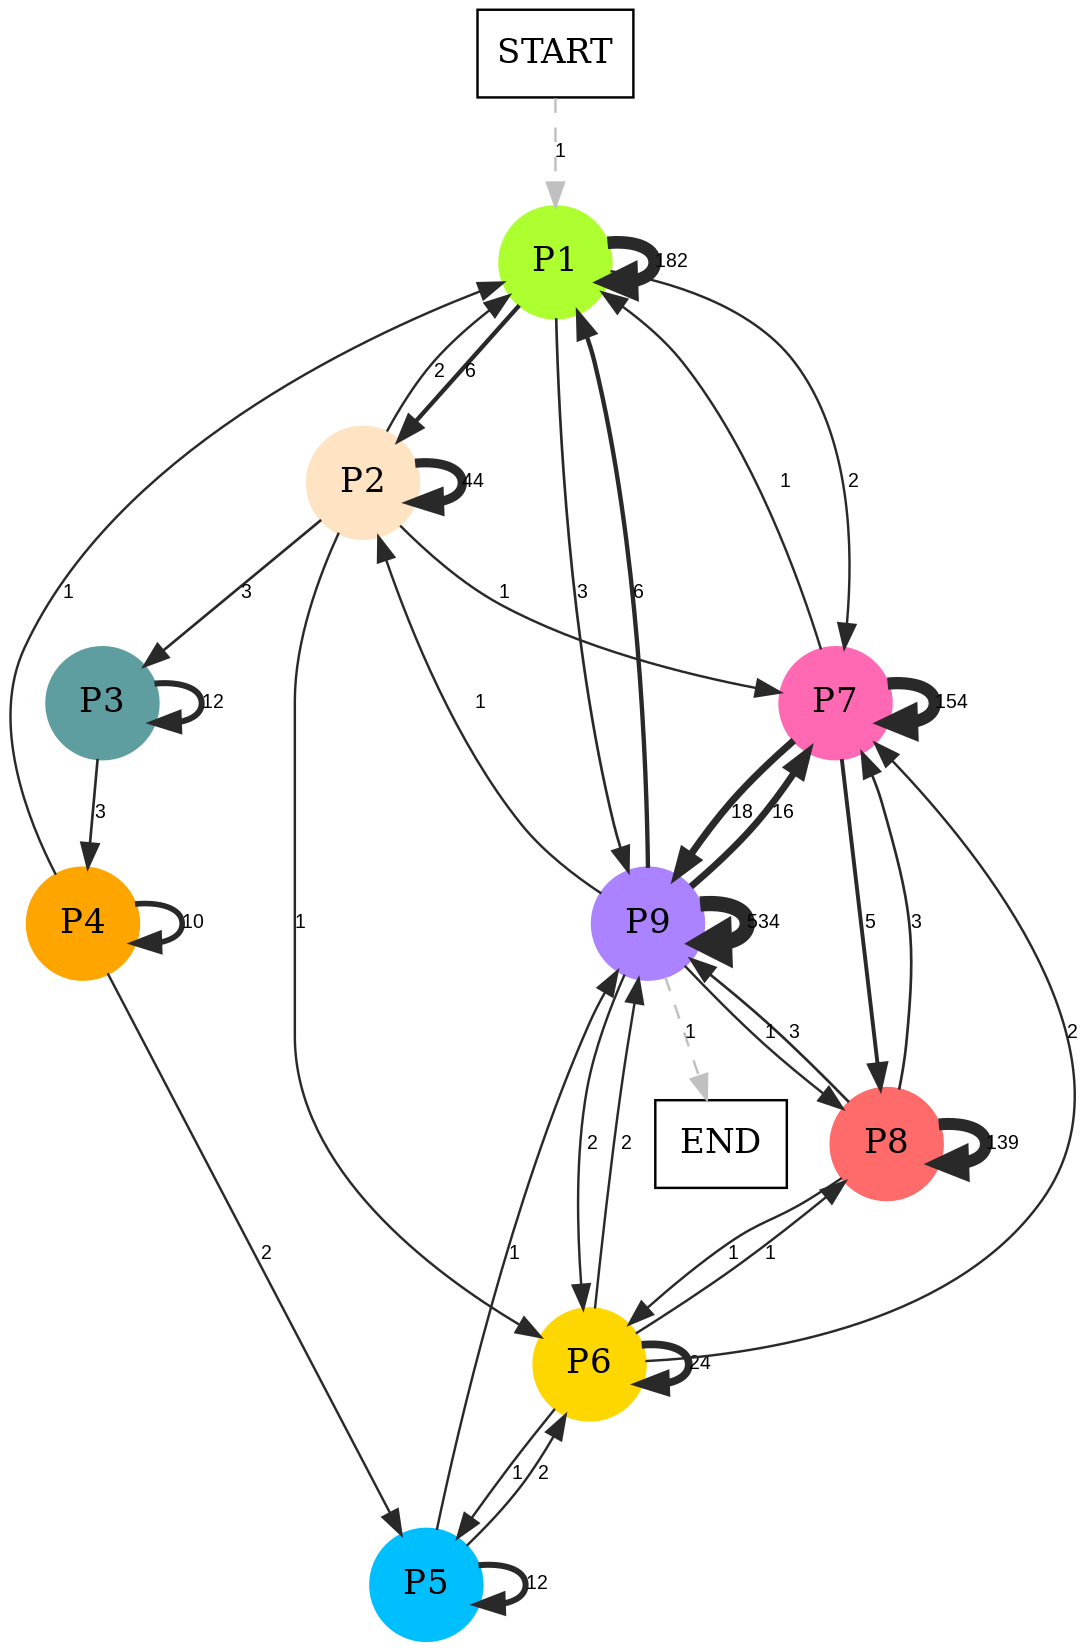
\includegraphics[width=0.47\textwidth]{DBA1516P2GG.png}}\qquad
\subfloat[Grafo que muestra la exploración de los problemas, considerando si un problema ha sido resuelto (\texttt{OK}) o no (\texttt{FAIL}).]{\label{fig:DBA1516P2GG_states}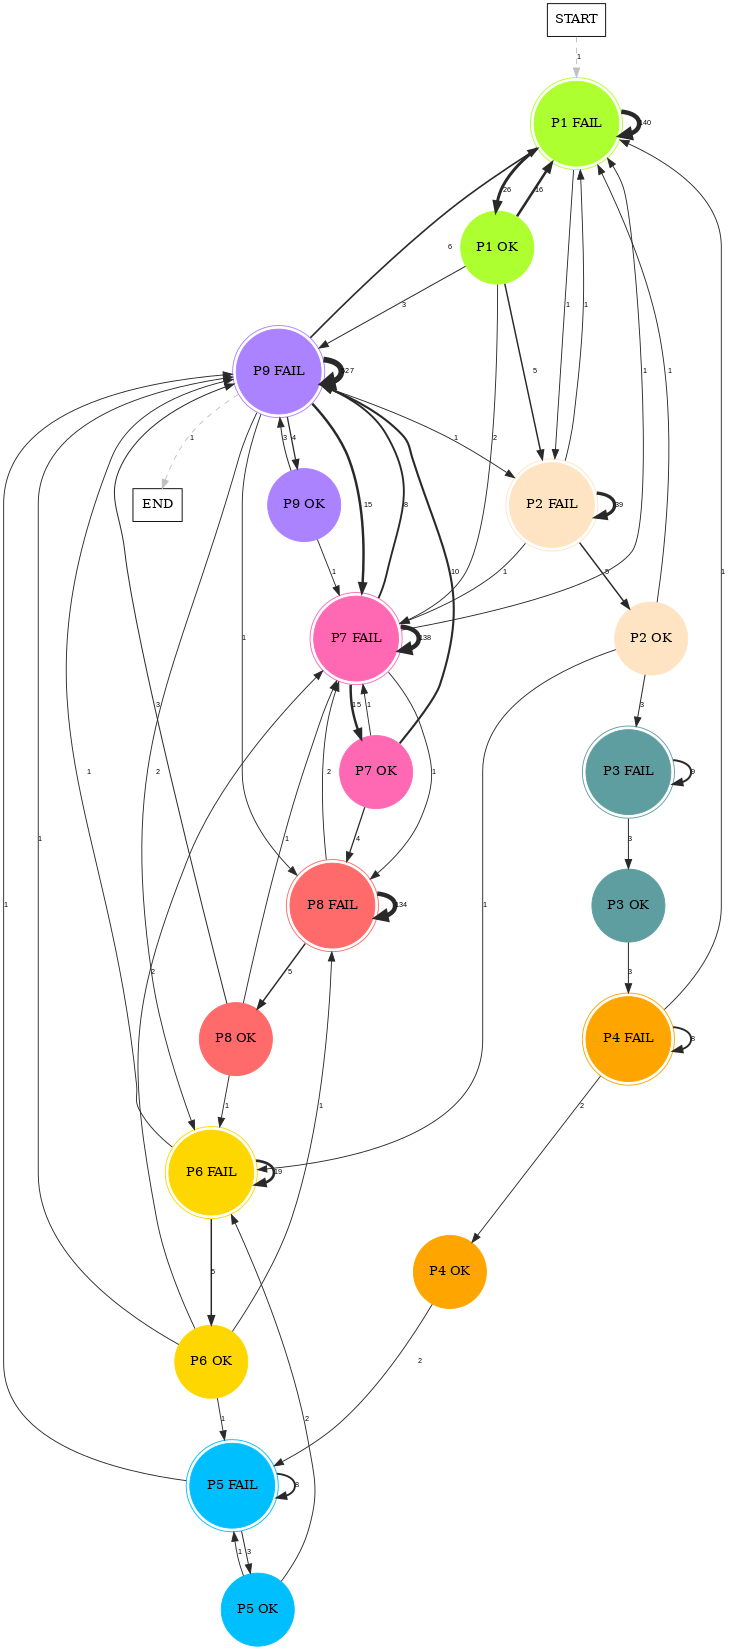
\includegraphics[width=0.47\textwidth]{DBA1516P2GG_states.png}}
\caption{Leaning Path del grupo de prácticas \texttt{DBA1516P2GG}.}
\label{fig:laplacian}
\end{figure}

\subsection{El coeficiente \emph{DAG}}

El coeficiente DAG se calcula a partir de la matriz de adyacencia de un
grafo dirigido acíclico. Así pues, es la suma de dos componentes, ponderadas
por $0.2$ y $0.8$ respectivamente.

La primera de las componentes del coeficiente se calcula a partir de todos
los caminos del nodo inicial (\texttt{START}) al nodo final (\texttt{END}) de un grafo dirigido
acíclico dado. Así pues, se calcula la media de los problemas abiertos en
este tipo de caminos. Por ejemplo, dado el grado de la Figura,
un posible camino es \texttt{\{START,PROBLEM1-20,PROBLEM1-40,PROBLEM1-60,END\}}, en el que se abre un problema.

%\begin{figure}[H]
%\centering
%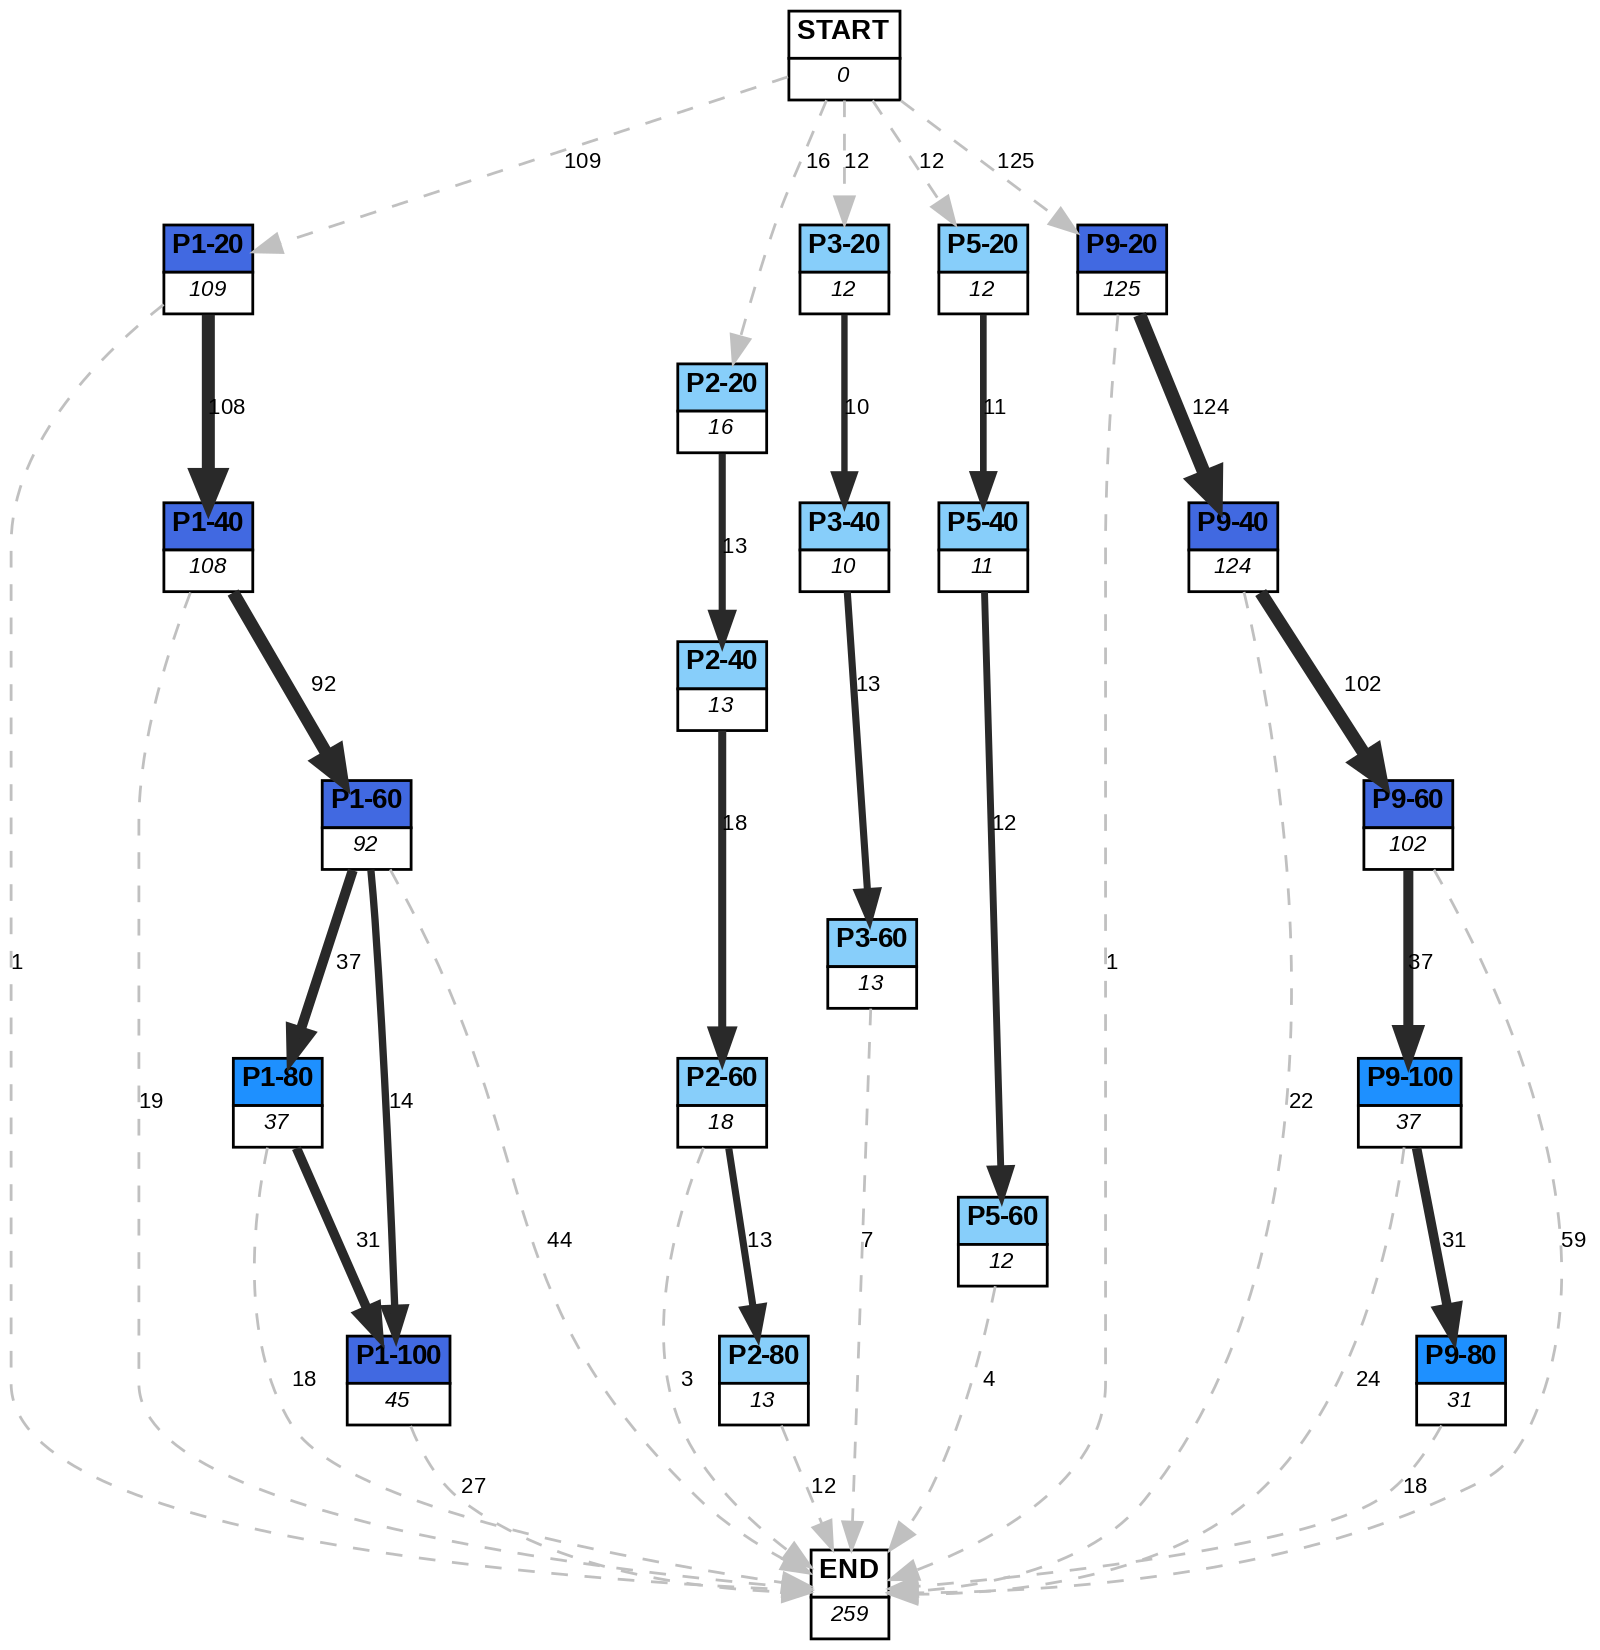
\includegraphics[width=\textwidth]{DBA2021P2GH.png}
%\caption{Grafo Dirigido Acíclico de ejemplo: grupo DBA2021GH}
%\label{fig:1}
%\end{figure}

Esta primera componente intenta captar el comportamiento de algunos grupos
que van saltando de problema en problema en la misma sesión, valorándolo
de manera negativa.

Por el contrario, la segunda componente no tiene ningún contenido semántico.
Ésta simplemente consiste en cálcular la desviación estándar de las componentes
de la matriz de adyacencia no nulas y dividirla por la media de dichas entradas.
En resumen, ésta segunda componente trata de ver cómo de balanceados están
los nodos de un grafo.

El pseudocódigo del cálculo de este coeficiente puede verse en el Algoritmo
\ref{alg:dag}.

\begin{algorithm}
\caption{Función encargada del cálculo del coeficiente DAG.}\label{alg:dag}
\begin{algorithmic}[1]
\Function{get\_coefficient}{}
\State $\texttt{coefficient} \gets 0$
\State $\texttt{problems} \gets \emptyset$ \Comment{Tiene el mismo tamaño que \texttt{paths}}
\For{$ i = 0 $ \textbf{to} $\texttt{paths.size()}$}
\State $\texttt{problems[i].add(num\_problems(paths[i]))}$
\EndFor
\If{$\texttt{paths.size()} == 0$}
\State $\texttt{coefficient} \gets 3$
\Else
\State $\texttt{mean} \gets \texttt{calculate\_mean(problems)}$
\State $\texttt{mean} \gets (\texttt{mean} - 1) / (9-1)$ \Comment{Normalización}
\State $\texttt{coefficient} \gets \texttt{coefficient} + 0.2 \cdot \texttt{mean}$
\State $\texttt{nonzero} \gets \emptyset$
\State $\texttt{mean\_frequency} \gets 0$
\State $\texttt{n} \gets 0$
\For{$\texttt{row}$ \textbf{in} $\texttt{frequency}$}
\For{$\texttt{element}$ \textbf{in} $\texttt{row}$}
\If{$\texttt{element} > 0$}
\State $\texttt{nonzero.add(element)}$
\State $\texttt{mean\_frequency} \gets \texttt{mean\_frequency} + \texttt{element}$
\State $\texttt{n} \gets \texttt{n}+1$
\EndIf
\EndFor
\EndFor
\State $\texttt{mean\_frequency} \gets \texttt{mean\_frequency}/\texttt{n}$
\State $\texttt{sum\_squares} \gets 0$
\For{$ i = 0 $ \textbf{to} $\texttt{n}$}
\State $\texttt{sum\_squares} \gets \texttt{sum\_squares} + (\texttt{nonzero[i]}-\texttt{mean\_frequency})^2$
\EndFor
\State $\texttt{variance} \gets \texttt{sum\_squares}/(\texttt{n}-1)$
\State $\texttt{std\_dev} \gets \texttt{sqrt(variance)}$
\State $\texttt{coefficient} \gets \texttt{coefficient} + 0.8 \cdot \texttt{std\_dev}/\texttt{mean\_frequency}$
\EndIf
\State \Return \texttt{coefficient}
\EndFunction
\end{algorithmic}
\end{algorithm}

Otra cosa que podría probarse es cambiar las ponderaciones del coeficiente
o ver qué pasa si se elimina la primera de las componentes del mismo ya que en la mayoría de las sesiones no es lo más frecuente saltar a otro problema.